% !TeX program = lualatex
\documentclass{article}
\usepackage[utf8]{inputenc}
\usepackage{amsmath}
\usepackage{tikz}
\usepackage{pgfplots, pgfplotstable}
\usetikzlibrary{calc}
\usepackage{pst-plot,pst-ode,multido}
\usepackage{derivative}

\pgfplotsset{ % Define a common style, so we don't repeat ourselves
	MyQuiver2D/.style={
		width=0.6\textwidth, % Overall width of the plot
		axis equal image, % Unit vectors for both axes have the same length
		view={0}{90}, % We need to use "3D" plots, but we set the view so we look at them from straight up
		xmin=-5.1, xmax=5.1, % Axis limits
		ymin=-5.1, ymax=5.1,
		domain=-5:5, y domain=-5:5, % Domain over which to evaluate the functions
		xtick={-5,-4,...,5}, ytick={-5,-4,...,5}, % Tick marks %
		samples=21, % How many arrows?
		cycle list={    % Plot styles
			gray,
			quiver={
				u={f(x,y)}, v={g(x,y)}, % End points of the arrows
				scale arrows=0.015,
				every arrow/.append style={
					-latex % Arrow tip
				},
			}\\
			red, samples=31, smooth, very thick, no markers, domain=-5:5 \\ % The plot style for the function
		}
	}
}

\definecolor[ps]{random}{rgb}{Rand Rand Rand}
\def\odeRHSone{
	x[0]*(x[0]-x[1])
	|
	x[1]*(2*x[0]-x[1])
}
\def\odeRHStwo{
	x[0]^2/x[1] - x[0]
	|
	x[0]^2 - 2*x[1]
}
\def\odeRHSfouraone{
	0-x[0]^2
	|
	-x[1]
}
\def\odeRHSfouratwo{
	1-x[0]^2
	|
	-x[1]
}
\def\odeRHSfourathree{
	-1-x[0]^2
	|
	-x[1]
}
\def\odeRHSfourbone{
	x[1]-2*x[0]
	|
	2+x[0]^2-x[1]
}
\def\odeRHSfourbtwo{
	x[1]-2*x[0]
	|
	1+x[0]^2-x[1]
}
\def\odeRHSfourbthree{
	x[1]-2*x[0]
	|
	0+x[0]^2-x[1]
}
\def\odeRHSfourbfour{
	x[1]-2*x[0]
	|
	-17/64+x[0]^2-x[1]
}
\def\odeRHSfourbfive{
	x[1]-2*x[0]
	|
	-1+x[0]^2-x[1]
}
\def\odeRHSfiveaone{
	0*x[0]-x[0]^2
	|
	-x[1]
}
\def\odeRHSfiveatwo{
	1*x[0]-x[0]^2
	|
	-x[1]
}
\def\odeRHSfiveathree{
	-1*x[0]-x[0]^2
	|
	-x[1]
}
\def\odeRHSfivebone{
	x[1]-2*x[0]
	|
	-x[1]+x[0]/(x[0]+1)
}
\def\odeRHSfivebtwo{
	x[1]-1*x[0]
	|
	-x[1]+x[0]/(x[0]+1)
}
\def\odeRHSfivebthree{
	x[1]-0*x[0]
	|
	-x[1]+x[0]/(x[0]+1)
}
\def\odeRHSfivebfour{
	x[1]--1*x[0]
	|
	-x[1]+x[0]/(x[0]+1)
}
\def\odeRHSfivebfive{
	x[1]--2*x[0]
	|
	-x[1]+x[0]/(x[0]+1)
}

\title{HW 7}
\author{Bowen Chen, Ravi Kini, Vaishnavi Kulkarni}
\date{March 2023}

\begin{document}
	
	\maketitle
	
	\begin{enumerate}
		\item 
		\begin{equation}
			\begin{split}
				\frac{dx}{dt} = 0 & = x(x - y) \\
				x^* & = 0, y^* \\
				\frac{dy}{dt} = 0 & = y(2x - y) \\
				y^* & = 0, 2x^* \\
				(x^*, y^*) & = (0,0) \\
				\operatorname{DF}(x,y) & = \begin{bmatrix} 2x - y & -x \\ 2y & 2x - 2y\end{bmatrix} \\
				(2x - y - \lambda)(2x - 2y - \lambda) + 2xy & = 0 \\
				\lambda & = \frac{4x - 3y \pm \sqrt{y(y-8x)}}{2} \\
				\lambda_{(0,0)} & = 0
			\end{split}
		\end{equation}
		
		Linear stability analysis does not reveal anything about the steady state $(0,0)$.
		
		The x-nullclines are in blue, and the y-nullclines in red.
		
		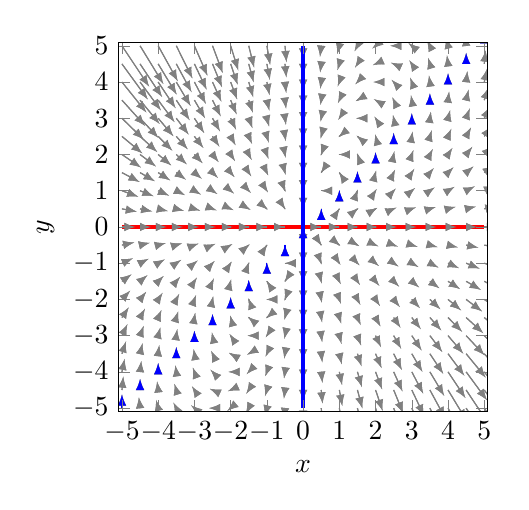
\begin{tikzpicture}[
			declare function={f(\x,\y) = \x*(\x-\y);},
			declare function={g(\x,\y) = \y*(2*\x-\y);}
			]
			\begin{axis}[
				MyQuiver2D,
				xlabel={$x$},ylabel={$y$}]
				\addplot3 (x,y,0);
				\addplot +[red] ({x},{0});
				\addplot3 (x,y,0);
				\addplot +[blue] ({0},{x});
				\addplot +[blue] ({x},{x});
			\end{axis}
		\end{tikzpicture}
		
		\psset{unit=0.5}
		\begin{pspicture}(-5.2,-5.2)(5.1,5.1)
			\psaxes[ticksize=0 4pt,axesstyle=frame,tickstyle=inner,
			Ox=-5,Oy=-5](-5,-5)(5,5)
			\psset{arrows=->,algebraic}
			\rput(-0.5,-6.5){$x$}
			\rput(-6.5,-0.5){$y$}
			\pstODEsolve[algebraicAll]{sol_1_1}{x[0] | x[1]}{0}{10}{100}{2 | 2}{\odeRHSone}
			\pstODEsolve[algebraicAll]{sol_1_2}{x[0] | x[1]}{0}{10}{100}{2 | 4}{\odeRHSone}
			\pstODEsolve[algebraicAll]{sol_2_1}{x[0] | x[1]}{0}{10}{100}{4 | 2}{\odeRHSone}
			\pstODEsolve[algebraicAll]{sol_n1_n1}{x[0] | x[1]}{0}{10}{100}{-2 | -2}{\odeRHSone}
			\pstODEsolve[algebraicAll]{sol_n1_n2}{x[0] | x[1]}{0}{10}{100}{-2 | -4}{\odeRHSone}
			\pstODEsolve[algebraicAll]{sol_n2_n1}{x[0] | x[1]}{0}{10}{100}{-4 | -2}{\odeRHSone}
			\pstODEsolve[algebraicAll]{sol_1_n1}{x[0] | x[1]}{0}{10}{100}{2 | -2}{\odeRHSone}
			\pstODEsolve[algebraicAll]{sol_n1_1}{x[0] | x[1]}{0}{10}{100}{-2 | 2}{\odeRHSone}
			
			
			\psset{arrows=->,linewidth=1pt}%
			\listplot[linecolor=random  ]{sol_1_1}
			\listplot[linecolor=random  ]{sol_1_2}
			\listplot[linecolor=random  ]{sol_2_1}
			\listplot[linecolor=random  ]{sol_n1_n1}
			\listplot[linecolor=random  ]{sol_n1_n2}
			\listplot[linecolor=random  ]{sol_n2_n1}
			\listplot[linecolor=random  ]{sol_1_n1}
			\listplot[linecolor=random  ]{sol_n1_1}
		\end{pspicture}
		\item
		\begin{enumerate}
			\item 
			\begin{equation}
				\begin{split}
					\frac{da}{dt} = 0 & = \frac{a^2}{h} - a \\
					a^* & = h^* \\
					\frac{dh}{dt} = 0 & = a^2 - 2h \\
					h^* & = \frac{{a^*}^2}{2} \\
					(a^*, h^*) & = (2,2) \\
					\operatorname{DF}(a,h) & = \begin{bmatrix} \frac{2a}{h} - 1 & -\frac{a^2}{h^2} \\ 2a & -1\end{bmatrix} \\
					(\frac{2a}{h} - 1 - \lambda)(-1 - \lambda) + \frac{2a^3}{h^2} & = 0 \\
					\lambda & = \frac{ah - h^2 \pm \sqrt{-a^2(2a-1)h^2}}{h^2} \\
					\lambda_{(2,2)} & = \pm i\sqrt{3}
				\end{split}
			\end{equation}
			The stable point $(2,2)$ is a center.
			
			The x-nullclines are in blue, and the y-nullclines in red.
			
			\begin{tikzpicture}[
				declare function={f(\x,\y) = \x^2/\y - \x;},
				declare function={g(\x,\y) = \x^2-2*\y;}
				]
				\begin{axis}[
					MyQuiver2D,
					xlabel={$a$},ylabel={$h$},xmin=0,xmax=5,ymin=0,ymax=5]
					\addplot3 (x,y,0);
					\addplot +[red] ({x},{x^2/2});
					\addplot3 (x,y,0);
					\addplot +[blue] ({x},{x});
				\end{axis}
			\end{tikzpicture}
			
			\psset{unit=2}
			\begin{pspicture}(0,0)(5.1,5.1)
				\psaxes[ticksize=0 4pt,axesstyle=frame,tickstyle=inner,
				Ox=0,Oy=0](0,0)(5,5)
				\psset{arrows=->,algebraic}
				\rput(2.5,-0.5){$a$}
				\rput(-0.5,2.5){$h$}
				\pstODEsolve[algebraicAll]{sol_1_1}{x[0] | x[1]}{0}{10}{100}{3 | 3}{\odeRHStwo}
				\pstODEsolve[algebraicAll]{sol_1_2}{x[0] | x[1]}{0}{10}{100}{2 | 4}{\odeRHStwo}
				\pstODEsolve[algebraicAll]{sol_2_1}{x[0] | x[1]}{0}{10}{100}{4 | 2}{\odeRHStwo}
				
				
				\psset{arrows=->,linewidth=1pt}%
				\listplot[linecolor=random  ]{sol_1_1}
				\listplot[linecolor=random  ]{sol_1_2}
				\listplot[linecolor=random  ]{sol_2_1}
			\end{pspicture}
			\\
			\\
			\begin{pspicture}(0,0)(10.1,5.1)
				\psaxes[ticksize=0 4pt,axesstyle=frame,tickstyle=inner,
				Ox=0,Oy=0](0,0)(10,5)
				\psset{arrows=->,algebraic}
				\rput(2.5,-0.5){$t$}
				\rput(-0.5,2.5){$a(t)$}
				\pstODEsolve[algebraicAll]{sol_1_1}{t | x[0]}{0}{10}{100}{3 | 3}{\odeRHStwo}
				
				
				\psset{arrows=->,linewidth=1pt}%
				\listplot[linecolor=random  ]{sol_1_1}
			\end{pspicture}
			
			\begin{pspicture}(0,0)(10.1,5.1)
				\psaxes[ticksize=0 4pt,axesstyle=frame,tickstyle=inner,
				Ox=0,Oy=0](0,0)(10,5)
				\psset{arrows=->,algebraic}
				\rput(2.5,-0.5){$t$}
				\rput(-0.5,2.5){$h(t)$}
				\pstODEsolve[algebraicAll]{sol_1_2}{t | x[1]}{0}{10}{100}{3 | 3}{\odeRHStwo}
				
				
				\psset{arrows=->,linewidth=1pt}%
				\listplot[linecolor=random  ]{sol_1_2}
			\end{pspicture}
			\\
			\\
		\end{enumerate}
		\item
		
		\begin{enumerate}
			\item [6.1.12.]
			\begin{equation}
				\begin{split}
					\frac{dx}{dt} = 0 & = \frac{x^2}{2}-2 \\
					x^* & = \pm 2 \\
					\frac{dy}{dt} = 0 & = -xy \\
					x^* & = 0, y^* = 0 \\
					(x^*, y^*) & = (\pm 2,0) \\
					\operatorname{DF}(x,y) & = \begin{bmatrix} x & 0 \\ -y & -x\end{bmatrix} \\
					-(x - \lambda)(x + \lambda) & = 0 \\
					\lambda & = \pm x \\
					\lambda_{(2,0)}, \lambda_{(-2,0)} & = \pm 2
				\end{split}
			\end{equation}
			
			The steady states $(2,0)$ and $(-2,0)$ are both saddle points.
			
			
			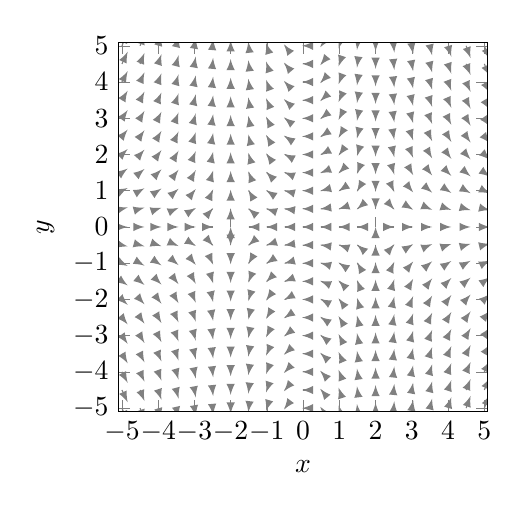
\begin{tikzpicture}[
				declare function={f(\x,\y) = \x^2/2-2;},
				declare function={g(\x,\y) = -\x*\y;}
				]
				\begin{axis}[
					MyQuiver2D,
					xlabel={$x$},ylabel={$y$}]
					\addplot3 (x,y,0);
				\end{axis}
			\end{tikzpicture}
			
			\begin{equation}
				\begin{split}
					\frac{dx}{dt} = 0 & = xy \\
					x^* & = 0, y^* = 0 \\
					\frac{dy}{dt} = 0 & = \frac{x^2}{2}-2 \\
					x^* & = \pm 2 \\
					(x^*, y^*) & = (\pm 2,0) \\
					\operatorname{DF}(x,y) & = \begin{bmatrix} y & x \\ x & 0\end{bmatrix} \\
					-(y - \lambda)\lambda + x^2 & = 0 \\
					\lambda & = \frac{y \pm \sqrt{y^2 + 4x^2}}{2} \\
					\lambda_{(2,0)}, \lambda_{(-2,0)} & = \pm 2
				\end{split}
			\end{equation}
			
			The steady states $(2,0)$ and $(-2,0)$ are both saddle points.
			
			
			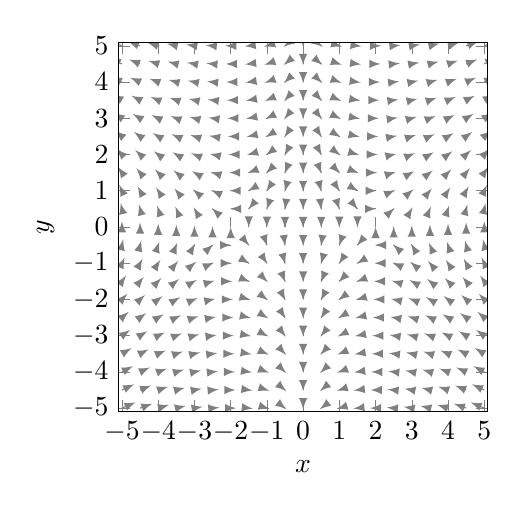
\begin{tikzpicture}[
				declare function={f(\x,\y) = \x*\y;},
				declare function={g(\x,\y) = \x^2/2-2;}
				]
				\begin{axis}[
					MyQuiver2D,
					xlabel={$x$},ylabel={$y$}]
					\addplot3 (x,y,0);
				\end{axis}
			\end{tikzpicture}
			\item [6.3.16.]
			\begin{enumerate}
				\item [a.] For $a = 0$:
				
				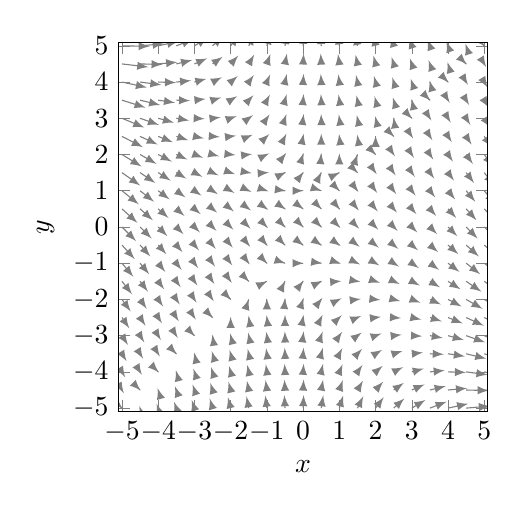
\begin{tikzpicture}[
					declare function={f(\x,\y) = 1+\x^2-\x*\y;},
					declare function={g(\x,\y) = \y^2-\x^2-1;}
					]
					\begin{axis}[
						MyQuiver2D,
						xlabel={$x$},ylabel={$y$}]
						\addplot3 (x,y,0);
					\end{axis}
				\end{tikzpicture}
				\item [b.] For $a = 1 > 0$, without loss of generality:
				
				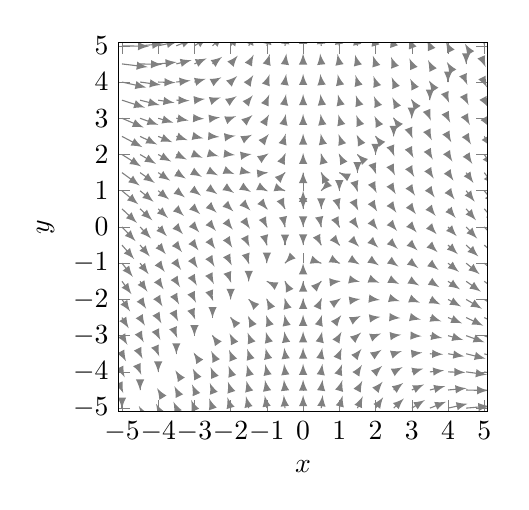
\begin{tikzpicture}[
					declare function={f(\x,\y) = 0+\x^2-\x*\y;},
					declare function={g(\x,\y) = \y^2-\x^2-1;}
					]
					\begin{axis}[
						MyQuiver2D,
						xlabel={$x$},ylabel={$y$}]
						\addplot3 (x,y,0);
					\end{axis}
				\end{tikzpicture}
				
				For $a = -1 < 0$, without loss of generality:
				
				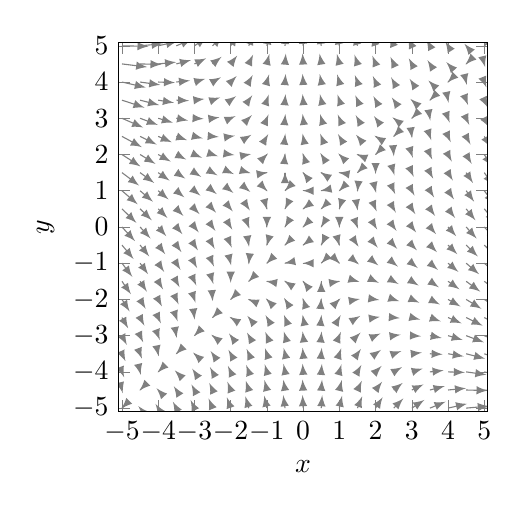
\begin{tikzpicture}[
					declare function={f(\x,\y) = -1+\x^2-\x*\y;},
					declare function={g(\x,\y) = \y^2-\x^2-1;}
					]
					\begin{axis}[
						MyQuiver2D,
						xlabel={$x$},ylabel={$y$}]
						\addplot3 (x,y,0);
					\end{axis}
				\end{tikzpicture}
			\end{enumerate}
		\end{enumerate}
		\item
		\begin{enumerate}
			\item 
			\begin{enumerate}
				\item 
				\begin{equation}
					\begin{split}
						\frac{dx}{dt} = 0 & = \mu - x^2 \\
						x^* & = \pm\sqrt{\mu} \\
						\frac{dy}{dt} = 0 & = -y \\
						y^* & = 0 \\
						(x^*, y^*) & = (\pm \sqrt{\mu},0) \\
						\operatorname{DF}(x,y) & = \begin{bmatrix} -2x & 0 \\ 0 & -1\end{bmatrix} \\
						(2x + \lambda)(1 + \lambda) & = 0 \\
						\lambda & = -1,-2x \\
						\lambda_{(\sqrt{\mu},0)} & = -1,-2\sqrt{\mu} \\
						\lambda_{(-\sqrt{\mu},0)} & = -1,2\sqrt{\mu}
					\end{split}
				\end{equation}
				
				If $-\infty < \mu < 0$, there are no steady states.
				
				If $\mu = 0$, there is a saddle node at $(0,0)$.
				
				If $0 < \mu < \infty$, there is a stable node at $(\sqrt{\mu},0)$ and saddle point at $(-\sqrt{\mu},0)$.
				\item
				\begin{tikzpicture}[scale=0.8]
					\begin{axis}[xmin=-5,xmax=5,ymin=-5,ymax=5,
						restrict x to domain=-5:5,restrict y to domain=-5:5,xlabel={$\mu$},ylabel={$x^*$}]
						\addplot[color=blue,solid,samples=100,domain=-5:5]{sqrt(x)};\addplot[color=blue,dashed,samples=100,domain=-5:5]{-sqrt(x)};
						\node[blue,below,align=center] at (axis cs:2,2.5){stable node};
						\node[blue,below,align=center] at (axis cs:2,-2.5){saddle point};
					\end{axis}
				\end{tikzpicture}
			
			A saddle-node bifurcation occurs at $\mu = 0$.
			\item The bifurcation point is at $\mu = 0$, where the steady state occurs at $(0,0)$. The eigenvalues for this point are:
			\begin{equation}
				\begin{split}
					\lambda & = -1,0
				\end{split}
			\end{equation}
			\item
			The x-nullclines are in blue, and the y-nullclines in red.
			
			
			For $\mu = 1$, without loss of generality:
			
			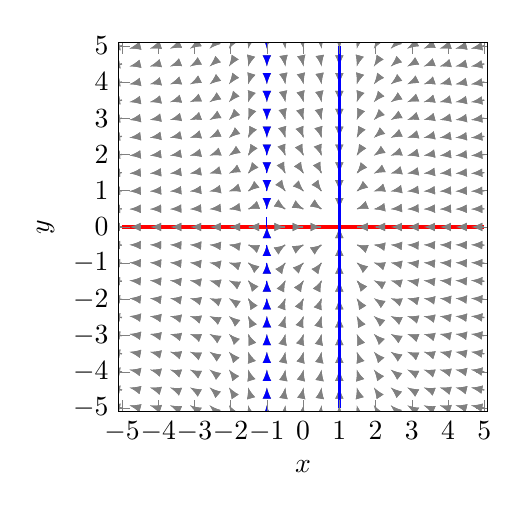
\begin{tikzpicture}[
				declare function={f(\x,\y) = 1-\x^2;},
				declare function={g(\x,\y) = -\y;}
				]
				\begin{axis}[
					MyQuiver2D,
					xlabel={$x$},ylabel={$y$}]
					\addplot3 (x,y,0);
					\addplot +[red] ({x},{0});
					\addplot3 (x,y,0);
					\addplot +[blue] ({1},{x});
					\addplot +[blue] ({-1},{x});
				\end{axis}
			\end{tikzpicture}
			
			\psset{unit=1}
			\begin{pspicture}(-5.2,-5.2)(5.1,5.1)
				\psaxes[ticksize=0 4pt,axesstyle=frame,tickstyle=inner,
				Ox=-5,Oy=-5](-5,-5)(5,5)
				\psset{arrows=->,algebraic}
				\rput(-0.5,-6.5){$x$}
				\rput(-6.5,-0.5){$y$}
				\pstODEsolve[algebraicAll]{sol_1_1}{x[0] | x[1]}{0}{2}{100}{2 | 2}{\odeRHSfouratwo}
				\pstODEsolve[algebraicAll]{sol_1_2}{x[0] | x[1]}{0}{2}{100}{0 | 2}{\odeRHSfouratwo}
				\pstODEsolve[algebraicAll]{sol_2_1}{x[0] | x[1]}{0}{2}{100}{0 | -2}{\odeRHSfouratwo}
				\pstODEsolve[algebraicAll]{sol_n1_n1}{x[0] | x[1]}{0}{0.2}{100}{-2 | -2}{\odeRHSfouratwo}
				\pstODEsolve[algebraicAll]{sol_1_n1}{x[0] | x[1]}{0}{2}{100}{2 | -2}{\odeRHSfouratwo}
				\pstODEsolve[algebraicAll]{sol_n1_1}{x[0] | x[1]}{0}{0.2}{100}{-2 | 2}{\odeRHSfouratwo}
				
				
				\psset{arrows=->,linewidth=1pt}%
				\listplot[linecolor=random  ]{sol_1_1}
				\listplot[linecolor=random  ]{sol_1_2}
				\listplot[linecolor=random  ]{sol_2_1}
				\listplot[linecolor=random  ]{sol_n1_n1}
				\listplot[linecolor=random  ]{sol_1_n1}
				\listplot[linecolor=random  ]{sol_n1_1}
			\end{pspicture}
			\\
			\\
			\\
			For $\mu = 0$:
			
			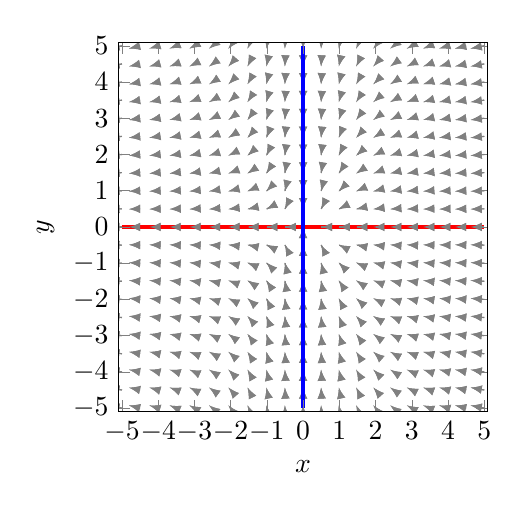
\begin{tikzpicture}[
				declare function={f(\x,\y) = 0-\x^2;},
				declare function={g(\x,\y) = -\y;}
				]
				\begin{axis}[
					MyQuiver2D,
					xlabel={$x$},ylabel={$y$}]
					\addplot3 (x,y,0);
					\addplot +[red] ({x},{0});
					\addplot3 (x,y,0);
					\addplot +[blue] ({0},{x});
				\end{axis}
			\end{tikzpicture}
			
			\psset{unit=1}
			\begin{pspicture}(-5.2,-5.2)(5.1,5.1)
				\psaxes[ticksize=0 4pt,axesstyle=frame,tickstyle=inner,
				Ox=-5,Oy=-5](-5,-5)(5,5)
				\psset{arrows=->,algebraic}
				\rput(-0.5,-6.5){$x$}
				\rput(-6.5,-0.5){$y$}
				\pstODEsolve[algebraicAll]{sol_1_1}{x[0] | x[1]}{0}{10}{100}{2 | 2}{\odeRHSfouraone}
				\pstODEsolve[algebraicAll]{sol_n1_n1}{x[0] | x[1]}{0}{0.2}{100}{-2 | -2}{\odeRHSfouraone}
				\pstODEsolve[algebraicAll]{sol_1_n1}{x[0] | x[1]}{0}{10}{100}{2 | -2}{\odeRHSfouraone}
				\pstODEsolve[algebraicAll]{sol_n1_1}{x[0] | x[1]}{0}{0.2}{100}{-2 | 2}{\odeRHSfouraone}
				
				
				\psset{arrows=->,linewidth=1pt}%
				\listplot[linecolor=random  ]{sol_1_1}
				\listplot[linecolor=random  ]{sol_n1_n1}
				\listplot[linecolor=random  ]{sol_1_n1}
				\listplot[linecolor=random  ]{sol_n1_1}
			\end{pspicture}
			\\
			\\
			\\
			For $\mu = -1$, without loss of generality:
			
			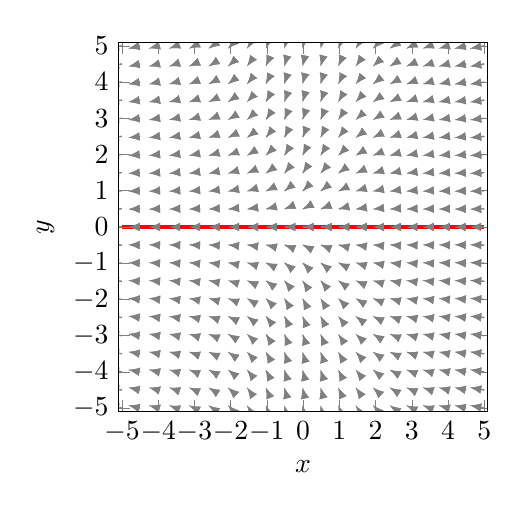
\begin{tikzpicture}[
				declare function={f(\x,\y) = -1-\x^2;},
				declare function={g(\x,\y) = -\y;}
				]
				\begin{axis}[
					MyQuiver2D,
					xlabel={$x$},ylabel={$y$}]
					\addplot3 (x,y,0);
					\addplot +[red] ({x},{0});
					\addplot3 (x,y,0);
				\end{axis}
			\end{tikzpicture}
			
			\psset{unit=1}
			\begin{pspicture}(-5.2,-5.2)(5.1,5.1)
				\psaxes[ticksize=0 4pt,axesstyle=frame,tickstyle=inner,
				Ox=-5,Oy=-5](-5,-5)(5,5)
				\psset{arrows=->,algebraic}
				\rput(-0.5,-6.5){$x$}
				\rput(-6.5,-0.5){$y$}
				\pstODEsolve[algebraicAll]{sol_1_1}{x[0] | x[1]}{0}{2}{100}{2 | 2}{\odeRHSfourathree}
				\pstODEsolve[algebraicAll]{sol_1_n1}{x[0] | x[1]}{0}{2}{100}{2 | -2}{\odeRHSfourathree}
				
				
				\psset{arrows=->,linewidth=1pt}%
				\listplot[linecolor=random  ]{sol_1_1}
				\listplot[linecolor=random  ]{sol_1_n1}
			\end{pspicture}
		\end{enumerate}
		\item
		\begin{enumerate}
			\item 
			\begin{equation}
				\begin{split}
					\frac{dx}{dt} = 0 & = y - 2x \\
					y^* & = 2x^* \\
					\frac{dy}{dt} = 0 & = \mu + x^2 - y \\
					y^* & = \mu + {x^*}^2 \\
					(x^*, y^*) & = (1 \pm \sqrt{1 - \mu},2 \pm 2\sqrt{1 - \mu}) \\
					\operatorname{DF}(x,y) & = \begin{bmatrix} -2 & 1 \\ 2x & -1\end{bmatrix} \\
					(-2-\lambda)(-1-\lambda) - 2x & = 0 \\
					\lambda & = \frac{-3\pm\sqrt{8x + 1}}{2} \\
					\lambda_{(1 + \sqrt{1 - \mu},2 + 2\sqrt{1 - \mu})} & = \frac{-3\pm\sqrt{8\sqrt{1 - \mu} + 9}}{2} \\
					\lambda_{(1 - \sqrt{1 - \mu},2 - 2\sqrt{1 - \mu})} & = \frac{-3\pm\sqrt{-8\sqrt{1 - \mu} + 9}}{2}
				\end{split}
			\end{equation}
		If $-\infty < \mu < -\frac{17}{64}$, there is a stable spiral at $(1 - \sqrt{1 - \mu},2 - 2\sqrt{1 - \mu})$ and a saddle point at $(1 + \sqrt{1 - \mu},2 + 2\sqrt{1 - \mu})$.
		
		If $\mu = -\frac{17}{64}$, there is a stable star node at $(-\frac{1}{8},-\frac{1}{4}$ and saddle point at $(\frac{17}{8},\frac{17}{4})$.
		
		If $-\frac{17}{64} < \mu < 1$, there is a stable node at $(1 - \sqrt{1 - \mu},2 - 2\sqrt{1 - \mu})$ and saddle point at $(1 + \sqrt{1 - \mu},2 + 2\sqrt{1 - \mu})$.
	
		If $\mu = 1$, there is a saddle node at $(1,2)$.
		
		If $1 < \mu < \infty$, there are no steady states. 
		\item
		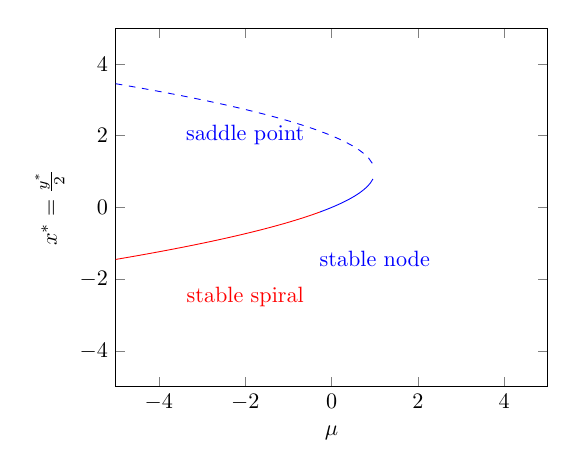
\begin{tikzpicture}[scale=0.8]
		\begin{axis}[xmin=-5,xmax=5,ymin=-5,ymax=5,
			restrict x to domain=-5:5,restrict y to domain=-5:5,xlabel={$\mu$},ylabel={$x^* = \frac{y^*}{2}$}]
			\addplot[color=blue,solid,samples=100,domain=-17/64:5]{1-sqrt(1-x)};
			\addplot[color=red,solid,samples=100,domain=-5:-17/64]{1-sqrt(1-x)};
			\addplot[color=blue,dashed,samples=100,domain=-5:5]{1+sqrt(1-x)};
			\node[blue,below,align=center] at (axis cs:1,-1){stable node};
			\node[red,below,align=center] at (axis cs:-2,-2){stable spiral};
			\node[blue,below,align=center] at (axis cs:-2,2.5){saddle point};
		\end{axis}
		\end{tikzpicture}
		
	A saddle-node bifurcation occurs at $\mu = 1$.
	
		
			\item The bifurcation point is at $\mu = 1$, where the steady state occurs at $(1,2)$. The eigenvalues for this point are:
			\begin{equation}
				\begin{split}
					\lambda & = -3,0
				\end{split}
			\end{equation}
			\item
			The x-nullclines are in blue, and the y-nullclines in red.
			
			For $\mu = 2$, without loss of generality:
			
			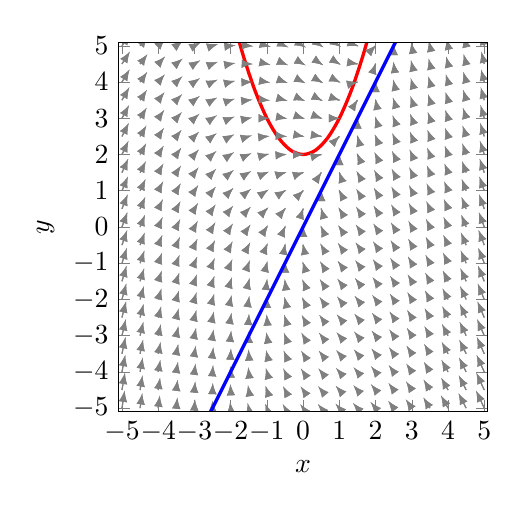
\begin{tikzpicture}[
				declare function={f(\x,\y) = \y-2*\x;},
				declare function={g(\x,\y) = 2+\x^2-\y;}
				]
				\begin{axis}[
					MyQuiver2D,
					xlabel={$x$},ylabel={$y$}]
					\addplot3 (x,y,0);
					\addplot +[red] {2+x^2};
					\addplot3 (x,y,0);
					\addplot +[blue] {2*x};
				\end{axis}
			\end{tikzpicture}
			
			\psset{unit=1}
			\begin{pspicture}(-5.2,-5.2)(5.1,5.1)
				\psaxes[ticksize=0 4pt,axesstyle=frame,tickstyle=inner,
				Ox=-5,Oy=-5](-5,-5)(5,5)
				\psset{arrows=->,algebraic}
				\rput(-0.5,-6.5){$x$}
				\rput(-6.5,-0.5){$y$}
				\pstODEsolve[algebraicAll]{sol_1_1}{x[0] | x[1]}{0}{2}{100}{2 | 2}{\odeRHSfourbone}
				\pstODEsolve[algebraicAll]{sol_1_2}{x[0] | x[1]}{0}{2}{100}{0 | 2}{\odeRHSfourbone}
				\pstODEsolve[algebraicAll]{sol_2_1}{x[0] | x[1]}{0}{2}{100}{0 | -2}{\odeRHSfourbone}
				\pstODEsolve[algebraicAll]{sol_n1_n1}{x[0] | x[1]}{0}{0.2}{100}{-2 | -2}{\odeRHSfourbone}
				\pstODEsolve[algebraicAll]{sol_1_n1}{x[0] | x[1]}{0}{2}{100}{2 | -2}{\odeRHSfourbone}
				\pstODEsolve[algebraicAll]{sol_n1_1}{x[0] | x[1]}{0}{0.2}{100}{-2 | 2}{\odeRHSfourbone}
				
				
				\psset{arrows=->,linewidth=1pt}%
				\listplot[linecolor=random  ]{sol_1_1}
				\listplot[linecolor=random  ]{sol_1_2}
				\listplot[linecolor=random  ]{sol_2_1}
				\listplot[linecolor=random  ]{sol_n1_n1}
				\listplot[linecolor=random  ]{sol_1_n1}
				\listplot[linecolor=random  ]{sol_n1_1}
			\end{pspicture}
			\\
			\\
			\\
			For $\mu = 1$:
			
			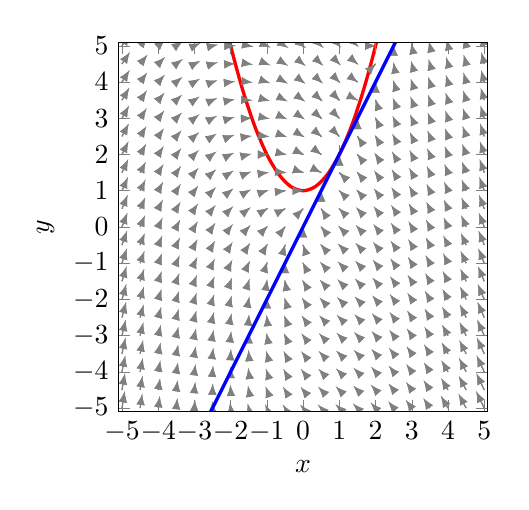
\begin{tikzpicture}[
				declare function={f(\x,\y) = \y-2*\x;},
				declare function={g(\x,\y) = 1+\x^2-\y;}
				]
				\begin{axis}[
					MyQuiver2D,
					xlabel={$x$},ylabel={$y$}]
					\addplot3 (x,y,0);
					\addplot +[red] {1+x^2};
					\addplot3 (x,y,0);
					\addplot +[blue] {2*x};
				\end{axis}
			\end{tikzpicture}
			
			\psset{unit=1}
			\begin{pspicture}(-5.2,-5.2)(5.1,5.1)
				\psaxes[ticksize=0 4pt,axesstyle=frame,tickstyle=inner,
				Ox=-5,Oy=-5](-5,-5)(5,5)
				\psset{arrows=->,algebraic}
				\rput(-0.5,-6.5){$x$}
				\rput(-6.5,-0.5){$y$}
				\pstODEsolve[algebraicAll]{sol_1_1}{x[0] | x[1]}{0}{2}{100}{2 | 2}{\odeRHSfourbtwo}
				\pstODEsolve[algebraicAll]{sol_1_2}{x[0] | x[1]}{0}{2}{100}{0 | 2}{\odeRHSfourbtwo}
				\pstODEsolve[algebraicAll]{sol_2_1}{x[0] | x[1]}{0}{2}{100}{0 | -2}{\odeRHSfourbtwo}
				\pstODEsolve[algebraicAll]{sol_n1_n1}{x[0] | x[1]}{0}{0.2}{100}{-2 | -2}{\odeRHSfourbtwo}
				\pstODEsolve[algebraicAll]{sol_1_n1}{x[0] | x[1]}{0}{2}{100}{2 | -2}{\odeRHSfourbtwo}
				\pstODEsolve[algebraicAll]{sol_n1_1}{x[0] | x[1]}{0}{0.2}{100}{-2 | 2}{\odeRHSfourbtwo}
				
				
				\psset{arrows=->,linewidth=1pt}%
				\listplot[linecolor=random  ]{sol_1_1}
				\listplot[linecolor=random  ]{sol_1_2}
				\listplot[linecolor=random  ]{sol_2_1}
				\listplot[linecolor=random  ]{sol_n1_n1}
				\listplot[linecolor=random  ]{sol_1_n1}
				\listplot[linecolor=random  ]{sol_n1_1}
			\end{pspicture}
			\\
			\\
			\\
			For $\mu = 0$, without loss of generality:
			
			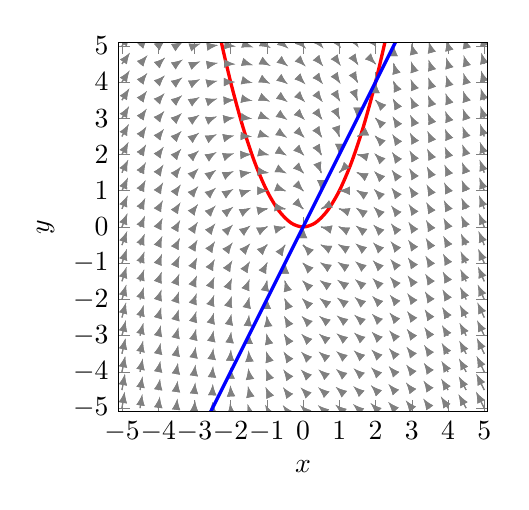
\begin{tikzpicture}[
				declare function={f(\x,\y) = \y-2*\x;},
				declare function={g(\x,\y) = 0+\x^2-\y;}
				]
				\begin{axis}[
					MyQuiver2D,
					xlabel={$x$},ylabel={$y$}]
					\addplot3 (x,y,0);
					\addplot +[red] {0+x^2};
					\addplot3 (x,y,0);
					\addplot +[blue] {2*x};
				\end{axis}
			\end{tikzpicture}
			
			\psset{unit=1}
			\begin{pspicture}(-5.2,-5.2)(5.1,5.1)
				\psaxes[ticksize=0 4pt,axesstyle=frame,tickstyle=inner,
				Ox=-5,Oy=-5](-5,-5)(5,5)
				\psset{arrows=->,algebraic}
				\rput(-0.5,-6.5){$x$}
				\rput(-6.5,-0.5){$y$}
				\pstODEsolve[algebraicAll]{sol_1_1}{x[0] | x[1]}{0}{2}{100}{2 | 2}{\odeRHSfourbthree}
				\pstODEsolve[algebraicAll]{sol_1_2}{x[0] | x[1]}{0}{2}{100}{0 | 2}{\odeRHSfourbthree}
				\pstODEsolve[algebraicAll]{sol_2_1}{x[0] | x[1]}{0}{2}{100}{0 | -2}{\odeRHSfourbthree}
				\pstODEsolve[algebraicAll]{sol_n1_n1}{x[0] | x[1]}{0}{0.2}{100}{-2 | -2}{\odeRHSfourbthree}
				\pstODEsolve[algebraicAll]{sol_1_n1}{x[0] | x[1]}{0}{2}{100}{2 | -2}{\odeRHSfourbthree}
				\pstODEsolve[algebraicAll]{sol_n1_1}{x[0] | x[1]}{0}{0.2}{100}{-2 | 2}{\odeRHSfourbthree}
				
				
				\psset{arrows=->,linewidth=1pt}%
				\listplot[linecolor=random  ]{sol_1_1}
				\listplot[linecolor=random  ]{sol_1_2}
				\listplot[linecolor=random  ]{sol_2_1}
				\listplot[linecolor=random  ]{sol_n1_n1}
				\listplot[linecolor=random  ]{sol_1_n1}
				\listplot[linecolor=random  ]{sol_n1_1}
			\end{pspicture}
			\\
			\\
			\\
			For $\mu = -\frac{17}{64}$:
			
			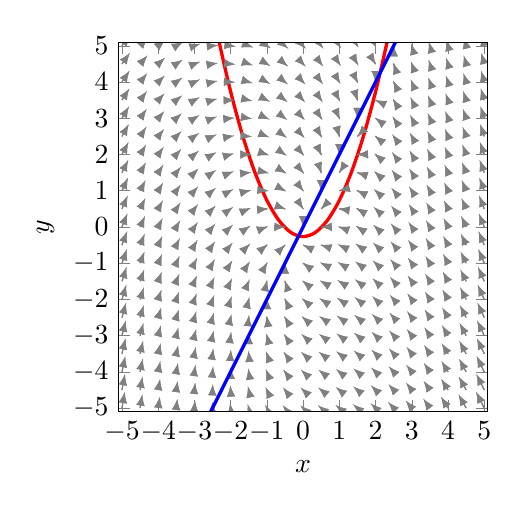
\begin{tikzpicture}[
				declare function={f(\x,\y) = \y-2*\x;},
				declare function={g(\x,\y) = -17/64+\x^2-\y;}
				]
				\begin{axis}[
					MyQuiver2D,
					xlabel={$x$},ylabel={$y$}]
					\addplot3 (x,y,0);
					\addplot +[red] {-17/64+x^2};
					\addplot3 (x,y,0);
					\addplot +[blue] {2*x};
				\end{axis}
			\end{tikzpicture}
			
			\psset{unit=1}
			\begin{pspicture}(-5.2,-5.2)(5.1,5.1)
				\psaxes[ticksize=0 4pt,axesstyle=frame,tickstyle=inner,
				Ox=-5,Oy=-5](-5,-5)(5,5)
				\psset{arrows=->,algebraic}
				\rput(-0.5,-6.5){$x$}
				\rput(-6.5,-0.5){$y$}
				\pstODEsolve[algebraicAll]{sol_1_1}{x[0] | x[1]}{0}{2}{100}{2 | 2}{\odeRHSfourbfour}
				\pstODEsolve[algebraicAll]{sol_1_2}{x[0] | x[1]}{0}{2}{100}{0 | 2}{\odeRHSfourbfour}
				\pstODEsolve[algebraicAll]{sol_2_1}{x[0] | x[1]}{0}{2}{100}{0 | -2}{\odeRHSfourbfour}
				\pstODEsolve[algebraicAll]{sol_n1_n1}{x[0] | x[1]}{0}{0.2}{100}{-2 | -2}{\odeRHSfourbfour}
				\pstODEsolve[algebraicAll]{sol_1_n1}{x[0] | x[1]}{0}{2}{100}{2 | -2}{\odeRHSfourbfour}
				\pstODEsolve[algebraicAll]{sol_n1_1}{x[0] | x[1]}{0}{0.2}{100}{-2 | 2}{\odeRHSfourbfour}
				
				
				\psset{arrows=->,linewidth=1pt}%
				\listplot[linecolor=random  ]{sol_1_1}
				\listplot[linecolor=random  ]{sol_1_2}
				\listplot[linecolor=random  ]{sol_2_1}
				\listplot[linecolor=random  ]{sol_n1_n1}
				\listplot[linecolor=random  ]{sol_1_n1}
				\listplot[linecolor=random  ]{sol_n1_1}
			\end{pspicture}
			\\
			\\
			\\
			For $\mu = -1$, without loss of generality:
			
			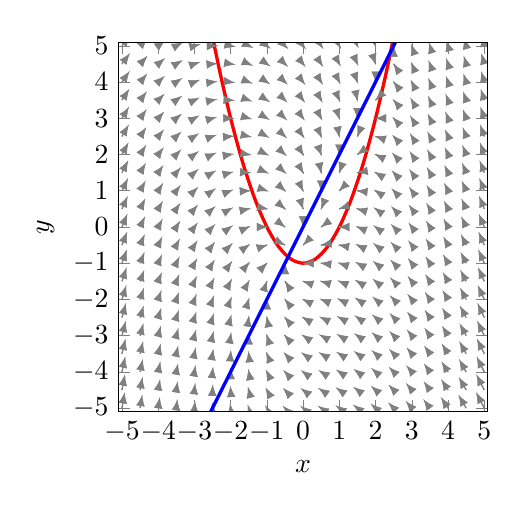
\begin{tikzpicture}[
				declare function={f(\x,\y) = \y-2*\x;},
				declare function={g(\x,\y) = -1+\x^2-\y;}
				]
				\begin{axis}[
					MyQuiver2D,
					xlabel={$x$},ylabel={$y$}]
					\addplot3 (x,y,0);
					\addplot +[red] {-1+x^2};
					\addplot3 (x,y,0);
					\addplot +[blue] {2*x};
				\end{axis}
			\end{tikzpicture}
			
			\psset{unit=1}
			\begin{pspicture}(-5.2,-5.2)(5.1,5.1)
				\psaxes[ticksize=0 4pt,axesstyle=frame,tickstyle=inner,
				Ox=-5,Oy=-5](-5,-5)(5,5)
				\psset{arrows=->,algebraic}
				\rput(-0.5,-6.5){$x$}
				\rput(-6.5,-0.5){$y$}
				\pstODEsolve[algebraicAll]{sol_1_1}{x[0] | x[1]}{0}{2}{100}{2 | 2}{\odeRHSfourbfive}
				\pstODEsolve[algebraicAll]{sol_1_2}{x[0] | x[1]}{0}{2}{100}{0 | 2}{\odeRHSfourbfive}
				\pstODEsolve[algebraicAll]{sol_2_1}{x[0] | x[1]}{0}{2}{100}{0 | -2}{\odeRHSfourbfive}
				\pstODEsolve[algebraicAll]{sol_n1_n1}{x[0] | x[1]}{0}{0.2}{100}{-2 | -2}{\odeRHSfourbfive}
				\pstODEsolve[algebraicAll]{sol_1_n1}{x[0] | x[1]}{0}{2}{100}{2 | -2}{\odeRHSfourbfive}
				\pstODEsolve[algebraicAll]{sol_n1_1}{x[0] | x[1]}{0}{0.2}{100}{-2 | 2}{\odeRHSfourbfive}
				
				
				\psset{arrows=->,linewidth=1pt}%
				\listplot[linecolor=random  ]{sol_1_1}
				\listplot[linecolor=random  ]{sol_1_2}
				\listplot[linecolor=random  ]{sol_2_1}
				\listplot[linecolor=random  ]{sol_n1_n1}
				\listplot[linecolor=random  ]{sol_1_n1}
				\listplot[linecolor=random  ]{sol_n1_1}
			\end{pspicture}
		\end{enumerate}
		\end{enumerate}
	\item
	\begin{enumerate}
		\item 
		\begin{enumerate}
			\item 
			\begin{equation}
				\begin{split}
					\frac{dx}{dt} = 0 & = \mu x - x^2 \\
					x^* & = 0,\mu \\
					\frac{dy}{dt} = 0 & = -y \\
					y^* & = 0 \\
					(x^*, y^*) & = (0,0),(\mu,0) \\
					\operatorname{DF}(x,y) & = \begin{bmatrix} \mu-2x & 0 \\ 0 & -1\end{bmatrix} \\
					-(\mu - 2x - \lambda)(1 + \lambda) & = 0 \\
					\lambda & = -1,\mu-2x \\
					\lambda_{(0,0)} & = -1,\mu \\
					\lambda_{(\mu,0)} & = -1,-\mu
				\end{split}
			\end{equation}
			
			If $-\infty < \mu < 0$, there is a stable node at $(0,0)$ and saddle point at $(\mu,0)$.
			
			If $\mu = 0$, there are saddle nodes at $(0,0)$ and $(\mu,0)$.
			
			If $0 < \mu < \infty$, there is a saddle point at $(0,0)$ and stable node at $(\mu,0)$.
			\item
			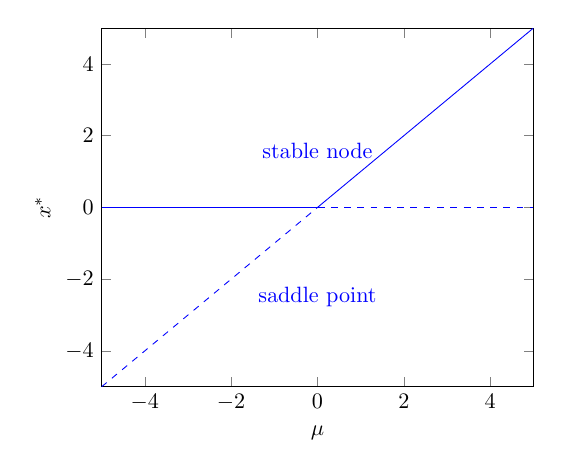
\begin{tikzpicture}[scale=0.8]
				\begin{axis}[xmin=-5,xmax=5,ymin=-5,ymax=5,
					restrict x to domain=-5:5,restrict y to domain=-5:5,xlabel={$\mu$},ylabel={$x^*$}]
					\addplot[color=blue,solid,samples=100,domain=-5:0]{0};
					\addplot[color=blue,dashed,samples=100,domain=-5:0]{x};
					\addplot[color=blue,dashed,samples=100,domain=0:5]{0};
					\addplot[color=blue,solid,samples=100,domain=0:5]{x};
					\node[blue,below,align=center] at (axis cs:0,2){stable node};
					\node[blue,below,align=center] at (axis cs:0,-2){saddle point};
				\end{axis}
			\end{tikzpicture}
			
			A transcritical bifurcation occurs at $\mu = 0$.
			\item The bifurcation point is at $\mu = 0$, where the steady state occurs at $(0,0)$. The eigenvalues for this point are:
			\begin{equation}
				\begin{split}
					\lambda & = -1,0
				\end{split}
			\end{equation}
			\item
			The x-nullclines are in blue, and the y-nullclines in red.
			
			
			For $\mu = 1$, without loss of generality:
			
			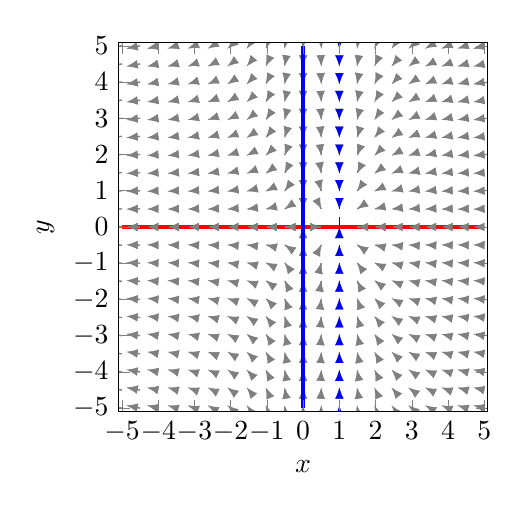
\begin{tikzpicture}[
				declare function={f(\x,\y) = 1*\x-\x^2;},
				declare function={g(\x,\y) = -\y;}
				]
				\begin{axis}[
					MyQuiver2D,
					xlabel={$x$},ylabel={$y$}]
					\addplot3 (x,y,0);
					\addplot +[red] ({x},{0});
					\addplot3 (x,y,0);
					\addplot +[blue] ({0},{x});
					\addplot +[blue] ({1},{x});
				\end{axis}
			\end{tikzpicture}
			
			\psset{unit=1}
			\begin{pspicture}(-5.2,-5.2)(5.1,5.1)
				\psaxes[ticksize=0 4pt,axesstyle=frame,tickstyle=inner,
				Ox=-5,Oy=-5](-5,-5)(5,5)
				\psset{arrows=->,algebraic}
				\rput(-0.5,-6.5){$x$}
				\rput(-6.5,-0.5){$y$}
				\pstODEsolve[algebraicAll]{sol_1_1}{x[0] | x[1]}{0}{2}{100}{2 | 2}{\odeRHSfiveatwo}
				\pstODEsolve[algebraicAll]{sol_1_2}{x[0] | x[1]}{0}{2}{100}{0 | 2}{\odeRHSfiveatwo}
				\pstODEsolve[algebraicAll]{sol_2_1}{x[0] | x[1]}{0}{2}{100}{0 | -2}{\odeRHSfiveatwo}
				\pstODEsolve[algebraicAll]{sol_n1_n1}{x[0] | x[1]}{0}{0.2}{100}{-2 | -2}{\odeRHSfiveatwo}
				\pstODEsolve[algebraicAll]{sol_1_n1}{x[0] | x[1]}{0}{2}{100}{2 | -2}{\odeRHSfiveatwo}
				\pstODEsolve[algebraicAll]{sol_n1_1}{x[0] | x[1]}{0}{0.2}{100}{-2 | 2}{\odeRHSfiveatwo}
				
				
				\psset{arrows=->,linewidth=1pt}%
				\listplot[linecolor=random  ]{sol_1_1}
				\listplot[linecolor=random  ]{sol_1_2}
				\listplot[linecolor=random  ]{sol_2_1}
				\listplot[linecolor=random  ]{sol_n1_n1}
				\listplot[linecolor=random  ]{sol_1_n1}
				\listplot[linecolor=random  ]{sol_n1_1}
			\end{pspicture}
			\\
			\\
			\\
			For $\mu = 0$:
			
			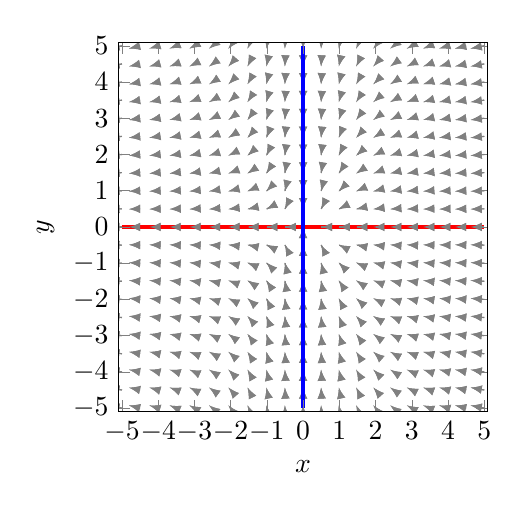
\begin{tikzpicture}[
				declare function={f(\x,\y) = 0*\x-\x^2;},
				declare function={g(\x,\y) = -\y;}
				]
				\begin{axis}[
					MyQuiver2D,
					xlabel={$x$},ylabel={$y$}]
					\addplot3 (x,y,0);
					\addplot +[red] ({x},{0});
					\addplot3 (x,y,0);
					\addplot +[blue] ({0},{x});
				\end{axis}
			\end{tikzpicture}
			
			\psset{unit=1}
			\begin{pspicture}(-5.2,-5.2)(5.1,5.1)
				\psaxes[ticksize=0 4pt,axesstyle=frame,tickstyle=inner,
				Ox=-5,Oy=-5](-5,-5)(5,5)
				\psset{arrows=->,algebraic}
				\rput(-0.5,-6.5){$x$}
				\rput(-6.5,-0.5){$y$}
				\pstODEsolve[algebraicAll]{sol_1_1}{x[0] | x[1]}{0}{10}{100}{2 | 2}{\odeRHSfiveaone}
				\pstODEsolve[algebraicAll]{sol_n1_n1}{x[0] | x[1]}{0}{0.2}{100}{-2 | -2}{\odeRHSfiveaone}
				\pstODEsolve[algebraicAll]{sol_1_n1}{x[0] | x[1]}{0}{10}{100}{2 | -2}{\odeRHSfiveaone}
				\pstODEsolve[algebraicAll]{sol_n1_1}{x[0] | x[1]}{0}{0.2}{100}{-2 | 2}{\odeRHSfiveaone}
				
				
				\psset{arrows=->,linewidth=1pt}%
				\listplot[linecolor=random  ]{sol_1_1}
				\listplot[linecolor=random  ]{sol_n1_n1}
				\listplot[linecolor=random  ]{sol_1_n1}
				\listplot[linecolor=random  ]{sol_n1_1}
			\end{pspicture}
			\\
			\\
			\\
			For $\mu = -1$, without loss of generality:
			
			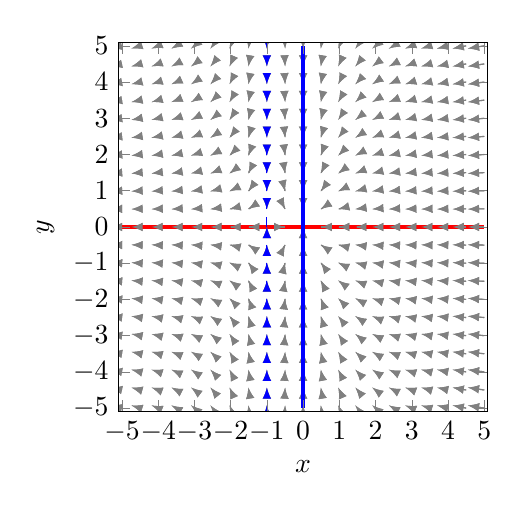
\begin{tikzpicture}[
				declare function={f(\x,\y) = -1*\x-\x^2;},
				declare function={g(\x,\y) = -\y;}
				]
				\begin{axis}[
					MyQuiver2D,
					xlabel={$x$},ylabel={$y$}]
					\addplot3 (x,y,0);
					\addplot +[red] ({x},{0});
					\addplot3 (x,y,0);
					\addplot +[blue] ({0},{x});
					\addplot +[blue] ({-1},{x});
				\end{axis}
			\end{tikzpicture}
			
			\psset{unit=1}
			\begin{pspicture}(-5.2,-5.2)(5.1,5.1)
				\psaxes[ticksize=0 4pt,axesstyle=frame,tickstyle=inner,
				Ox=-5,Oy=-5](-5,-5)(5,5)
				\psset{arrows=->,algebraic}
				\rput(-0.5,-6.5){$x$}
				\rput(-6.5,-0.5){$y$}
				\pstODEsolve[algebraicAll]{sol_1_1}{x[0] | x[1]}{0}{2}{100}{2 | 2}{\odeRHSfiveathree}
				\pstODEsolve[algebraicAll]{sol_1_n1}{x[0] | x[1]}{0}{2}{100}{2 | -2}{\odeRHSfiveathree}
				\pstODEsolve[algebraicAll]{sol_n1_1}{x[0] | x[1]}{0}{0.2}{100}{-2 | 2}{\odeRHSfiveathree}
				\pstODEsolve[algebraicAll]{sol_n1_n1}{x[0] | x[1]}{0}{0.2}{100}{-2 | -2}{\odeRHSfiveathree}
				
				
				\psset{arrows=->,linewidth=1pt}%
				\listplot[linecolor=random  ]{sol_1_1}
				\listplot[linecolor=random  ]{sol_1_n1}
				\listplot[linecolor=random  ]{sol_n1_1}
				\listplot[linecolor=random  ]{sol_n1_n1}
			\end{pspicture}
		\end{enumerate}
		\item
		\begin{enumerate}
			\item 
			\begin{equation}
				\begin{split}
					\frac{dx}{dt} = 0 & = y - \mu x \\
					y^* & = \mu x^* \\
					\frac{dy}{dt} = 0 & = - y + \frac{x}{x + 1} \\
					y^* & = \frac{x^*}{x^* + 1} \\
					(x^*, y^*) & = (0,0), (\frac{1-\mu}{\mu},1-\mu) \\
					\operatorname{DF}(x,y) & = \begin{bmatrix} -\mu & 1 \\ \frac{1}{(x+1)^2} & -1\end{bmatrix} \\
					(-\mu-\lambda)(-1-\lambda) - \frac{1}{(x+1)^2} & = 0 \\
					\lambda_{(0,0)} & = \frac{-1-\mu\pm\sqrt{\mu^2-2\mu+5}}{2} \\
					\lambda_{(\frac{1-\mu}{\mu},1-\mu)} & = \frac{-1-\mu\pm\sqrt{5\mu^2-2\mu+1}}{2} \\
				\end{split}
			\end{equation}
			If $-\infty < \mu < -1$, there is a saddle point at $(0,0)$ and $(\frac{1-\mu}{\mu},1-\mu)$.
			
			If $\mu = -1$, there is a saddle point at $(0,0)$ and $(-2,2)$.
			
			If $-1 < \mu < 1$, there is a saddle point at $(0,0)$ and a stable node at $(\frac{1-\mu}{\mu},1-\mu)$.
			
			If $\mu = 1$, there is a saddle node at $(0,0)$.
			
			If $1 < \mu < \infty$, there is a stable node at $(0,0)$ and a saddle point at $(\frac{1-\mu}{\mu},1-\mu)$. 
			\item
			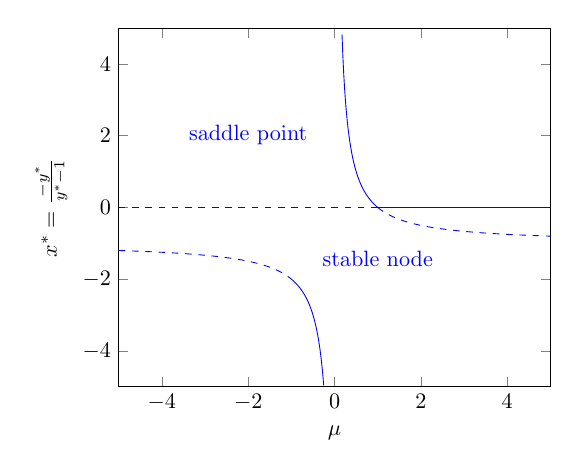
\begin{tikzpicture}[scale=0.8]
				\begin{axis}[xmin=-5,xmax=5,ymin=-5,ymax=5,
					restrict x to domain=-5:5,restrict y to domain=-5:5,xlabel={$\mu$},ylabel={$x^* = \frac{-y^*}{y^*-1}$}]
						\addplot[color=blue,solid,samples=100,domain=-1:1]{(1-x)/x};
						\addplot[color=blue,dashed,samples=100,domain=1:5]{(1-x)/x};
						\addplot[color=blue,dashed,samples=100,domain=-5:-1]{(1-x)/x};
					\addplot[color=blue,dashed,samples=100,domain=-5:1]{0};
					\addplot[color=blue,solid,samples=100,domain=1:5]{0};
					\node[blue,below,align=center] at (axis cs:1,-1){stable node};
					\node[blue,below,align=center] at (axis cs:-2,2.5){saddle point};
				\end{axis}
			\end{tikzpicture}
			
			A transcritical bifurcation occurs at $\mu = 1$.
			\item The bifurcation points is at $\mu = 1$, where the steady state occurs at $(0,0)$. The eigenvalues for this point are:
			\begin{equation}
				\begin{split}
					\lambda & = -2,0
				\end{split}
			\end{equation}
			\item
			The x-nullclines are in blue, and the y-nullclines in red.
			
			For $\mu = 2$, without loss of generality:
			
			\begin{tikzpicture}[
				declare function={f(\x,\y) = \y-2*\x;},
				declare function={g(\x,\y) = -\y+\x/(\x+1);}
				]
				\begin{axis}[
					MyQuiver2D,
					xlabel={$x$},ylabel={$y$}]
					\addplot3 (x,y,0);
					\addplot +[red] ({x},{x/(x+1)});
					\addplot3 (x,y,0);
					\addplot +[blue] ({x},{2*x});
				\end{axis}
			\end{tikzpicture}
			
			\psset{unit=1}
			\begin{pspicture}(-5.2,-5.2)(5.1,5.1)
				\psaxes[ticksize=0 4pt,axesstyle=frame,tickstyle=inner,
				Ox=-5,Oy=-5](-5,-5)(5,5)
				\psset{arrows=->,algebraic}
				\rput(-0.5,-6.5){$x$}
				\rput(-6.5,-0.5){$y$}
				\pstODEsolve[algebraicAll]{sol_1_1}{x[0] | x[1]}{0}{2}{100}{2 | 2}{\odeRHSfivebone}
				\pstODEsolve[algebraicAll]{sol_1_2}{x[0] | x[1]}{0}{2}{100}{0 | 2}{\odeRHSfivebone}
				\pstODEsolve[algebraicAll]{sol_2_1}{x[0] | x[1]}{0}{2}{100}{0 | -2}{\odeRHSfivebone}
				\pstODEsolve[algebraicAll]{sol_n1_n1}{x[0] | x[1]}{0}{0.2}{100}{-2 | -2}{\odeRHSfivebone}
				\pstODEsolve[algebraicAll]{sol_1_n1}{x[0] | x[1]}{0}{2}{100}{2 | -2}{\odeRHSfivebone}
				\pstODEsolve[algebraicAll]{sol_n1_1}{x[0] | x[1]}{0}{0.2}{100}{-2 | 2}{\odeRHSfivebone}
				
				
				\psset{arrows=->,linewidth=1pt}%
				\listplot[linecolor=random  ]{sol_1_1}
				\listplot[linecolor=random  ]{sol_1_2}
				\listplot[linecolor=random  ]{sol_2_1}
				\listplot[linecolor=random  ]{sol_n1_n1}
				\listplot[linecolor=random  ]{sol_1_n1}
				\listplot[linecolor=random  ]{sol_n1_1}
			\end{pspicture}
			\\
			\\
			\\
			For $\mu = 1$:
			
			\begin{tikzpicture}[
				declare function={f(\x,\y) = \y-1*\x;},
				declare function={g(\x,\y) = -\y+\x/(\x+1);}
				]
				\begin{axis}[
					MyQuiver2D,
					xlabel={$x$},ylabel={$y$}]
					\addplot3 (x,y,0);
					\addplot +[red] ({x},{x/(x+1)});
					\addplot3 (x,y,0);
					\addplot +[blue] ({x},{1*x});
				\end{axis}
			\end{tikzpicture}
			
			\psset{unit=1}
			\begin{pspicture}(-5.2,-5.2)(5.1,5.1)
				\psaxes[ticksize=0 4pt,axesstyle=frame,tickstyle=inner,
				Ox=-5,Oy=-5](-5,-5)(5,5)
				\psset{arrows=->,algebraic}
				\rput(-0.5,-6.5){$x$}
				\rput(-6.5,-0.5){$y$}
				\pstODEsolve[algebraicAll]{sol_1_1}{x[0] | x[1]}{0}{2}{100}{2 | 2}{\odeRHSfivebtwo}
				\pstODEsolve[algebraicAll]{sol_1_2}{x[0] | x[1]}{0}{2}{100}{0 | 2}{\odeRHSfivebtwo}
				\pstODEsolve[algebraicAll]{sol_2_1}{x[0] | x[1]}{0}{2}{100}{0 | -2}{\odeRHSfivebtwo}
				\pstODEsolve[algebraicAll]{sol_n1_n1}{x[0] | x[1]}{0}{0.2}{100}{-2 | -2}{\odeRHSfivebtwo}
				\pstODEsolve[algebraicAll]{sol_1_n1}{x[0] | x[1]}{0}{2}{100}{2 | -2}{\odeRHSfivebtwo}
				\pstODEsolve[algebraicAll]{sol_n1_1}{x[0] | x[1]}{0}{0.2}{100}{-2 | 2}{\odeRHSfivebtwo}
				
				
				\psset{arrows=->,linewidth=1pt}%
				\listplot[linecolor=random  ]{sol_1_1}
				\listplot[linecolor=random  ]{sol_1_2}
				\listplot[linecolor=random  ]{sol_2_1}
				\listplot[linecolor=random  ]{sol_n1_n1}
				\listplot[linecolor=random  ]{sol_1_n1}
				\listplot[linecolor=random  ]{sol_n1_1}
			\end{pspicture}
			\\
			\\
			\\
			For $\mu = 0$, without loss of generality:
			
			\begin{tikzpicture}[
				declare function={f(\x,\y) = \y-0*\x;},
				declare function={g(\x,\y) = -\y+\x/(\x+1);}
				]
				\begin{axis}[
					MyQuiver2D,
					xlabel={$x$},ylabel={$y$}]
					\addplot3 (x,y,0);
					\addplot +[red] ({x},{x/(x+1)});
					\addplot3 (x,y,0);
					\addplot +[blue] ({x},{0*x});
				\end{axis}
			\end{tikzpicture}
			
			\psset{unit=1}
			\begin{pspicture}(-5.2,-5.2)(5.1,5.1)
				\psaxes[ticksize=0 4pt,axesstyle=frame,tickstyle=inner,
				Ox=-5,Oy=-5](-5,-5)(5,5)
				\psset{arrows=->,algebraic}
				\rput(-0.5,-6.5){$x$}
				\rput(-6.5,-0.5){$y$}
				\pstODEsolve[algebraicAll]{sol_1_1}{x[0] | x[1]}{0}{2}{100}{2 | 2}{\odeRHSfivebthree}
				\pstODEsolve[algebraicAll]{sol_1_2}{x[0] | x[1]}{0}{2}{100}{0 | 2}{\odeRHSfivebthree}
				\pstODEsolve[algebraicAll]{sol_2_1}{x[0] | x[1]}{0}{2}{100}{0 | -2}{\odeRHSfivebthree}
				\pstODEsolve[algebraicAll]{sol_n1_n1}{x[0] | x[1]}{0}{0.2}{100}{-2 | -2}{\odeRHSfivebthree}
				\pstODEsolve[algebraicAll]{sol_1_n1}{x[0] | x[1]}{0}{2}{100}{2 | -2}{\odeRHSfivebthree}
				\pstODEsolve[algebraicAll]{sol_n1_1}{x[0] | x[1]}{0}{0.2}{100}{-2 | 2}{\odeRHSfivebthree}
				
				
				\psset{arrows=->,linewidth=1pt}%
				\listplot[linecolor=random  ]{sol_1_1}
				\listplot[linecolor=random  ]{sol_1_2}
				\listplot[linecolor=random  ]{sol_2_1}
				\listplot[linecolor=random  ]{sol_n1_n1}
				\listplot[linecolor=random  ]{sol_1_n1}
				\listplot[linecolor=random  ]{sol_n1_1}
			\end{pspicture}
			\\
			\\
			\\
			For $\mu = -1$:
			
		\begin{tikzpicture}[
			declare function={f(\x,\y) = \y--1*\x;},
			declare function={g(\x,\y) = -\y+\x/(\x+1);}
			]
			\begin{axis}[
				MyQuiver2D,
				xlabel={$x$},ylabel={$y$}]
				\addplot3 (x,y,0);
				\addplot +[red] ({x},{x/(x+1)});
				\addplot3 (x,y,0);
				\addplot +[blue] ({x},{-1*x});
			\end{axis}
		\end{tikzpicture}
			
			\psset{unit=1}
			\begin{pspicture}(-5.2,-5.2)(5.1,5.1)
				\psaxes[ticksize=0 4pt,axesstyle=frame,tickstyle=inner,
				Ox=-5,Oy=-5](-5,-5)(5,5)
				\psset{arrows=->,algebraic}
				\rput(-0.5,-6.5){$x$}
				\rput(-6.5,-0.5){$y$}
				\pstODEsolve[algebraicAll]{sol_1_1}{x[0] | x[1]}{0}{0.2}{100}{2 | 2}{\odeRHSfivebfour}
				\pstODEsolve[algebraicAll]{sol_1_2}{x[0] | x[1]}{0}{0.2}{100}{0 | 2}{\odeRHSfivebfour}
				\pstODEsolve[algebraicAll]{sol_2_1}{x[0] | x[1]}{0}{2}{100}{0 | -2}{\odeRHSfivebfour}
				\pstODEsolve[algebraicAll]{sol_n1_n1}{x[0] | x[1]}{0}{0.2}{100}{-2 | -2}{\odeRHSfivebfour}
				\pstODEsolve[algebraicAll]{sol_1_n1}{x[0] | x[1]}{0}{0.2}{100}{2 | -2}{\odeRHSfivebfour}
				\pstODEsolve[algebraicAll]{sol_n1_1}{x[0] | x[1]}{0}{0.2}{100}{-2 | 2}{\odeRHSfivebfour}
				
				
				\psset{arrows=->,linewidth=1pt}%
				\listplot[linecolor=random  ]{sol_1_1}
				\listplot[linecolor=random  ]{sol_1_2}
				\listplot[linecolor=random  ]{sol_2_1}
				\listplot[linecolor=random  ]{sol_n1_n1}
				\listplot[linecolor=random  ]{sol_1_n1}
				\listplot[linecolor=random  ]{sol_n1_1}
			\end{pspicture}
			\\
			\\
			\\
			For $\mu = -2$, without loss of generality:
			
			\begin{tikzpicture}[
				declare function={f(\x,\y) = \y--2*\x;},
				declare function={g(\x,\y) = -\y+\x/(\x+1);}
				]
				\begin{axis}[
					MyQuiver2D,
					xlabel={$x$},ylabel={$y$}]
					\addplot3 (x,y,0);
					\addplot +[red] ({x},{x/(x+1)});
					\addplot3 (x,y,0);
					\addplot +[blue] ({x},{-2*x});
				\end{axis}
			\end{tikzpicture}
			
			\psset{unit=1}
			\begin{pspicture}(-5.2,-5.2)(5.1,5.1)
				\psaxes[ticksize=0 4pt,axesstyle=frame,tickstyle=inner,
				Ox=-5,Oy=-5](-5,-5)(5,5)
				\psset{arrows=->,algebraic}
				\rput(-0.5,-6.5){$x$}
				\rput(-6.5,-0.5){$y$}
				\pstODEsolve[algebraicAll]{sol_1_1}{x[0] | x[1]}{0}{0.2}{100}{2 | 2}{\odeRHSfivebfive}
				\pstODEsolve[algebraicAll]{sol_1_2}{x[0] | x[1]}{0}{0.2}{100}{0 | 2}{\odeRHSfivebfive}
				\pstODEsolve[algebraicAll]{sol_2_1}{x[0] | x[1]}{0}{2}{100}{0 | -2}{\odeRHSfivebfive}
				\pstODEsolve[algebraicAll]{sol_n1_n1}{x[0] | x[1]}{0}{0.2}{100}{-2 | -2}{\odeRHSfivebfive}
				\pstODEsolve[algebraicAll]{sol_1_n1}{x[0] | x[1]}{0}{0.2}{100}{2 | -2}{\odeRHSfivebfive}
				\pstODEsolve[algebraicAll]{sol_n1_1}{x[0] | x[1]}{0}{0.2}{100}{-2 | 2}{\odeRHSfivebfive}
				
				
				\psset{arrows=->,linewidth=1pt}%
				\listplot[linecolor=random  ]{sol_1_1}
				\listplot[linecolor=random  ]{sol_1_2}
				\listplot[linecolor=random  ]{sol_2_1}
				\listplot[linecolor=random  ]{sol_n1_n1}
				\listplot[linecolor=random  ]{sol_1_n1}
				\listplot[linecolor=random  ]{sol_n1_1}
			\end{pspicture}
		\end{enumerate}
	\end{enumerate}
	\end{enumerate}
	
\end{document}
